\subsection{Модель проектирования MVVM}
MVVM (Model-View-ViewModel) является архитектурным шаблоном проектирования, основанным на идее разделения ответственности в приложении для обеспечения модульности, упрощения тестирования и поддержки. MVVM был разработан как альтернатива прямому управлению пользовательским интерфейсом из кода, что может привести к сложным и плохо структурированным приложениям. Он получил широкое распространение, особенно в области разработки клиентских приложений на платформе .NET, и является ключевым паттерном для разработки мобильных приложений на MAUI \cite{MVVM}. 

MVVM состоит из трех основных компонентов:
\begin{itemize}
\item Модель (Model): представляет собой объекты данных и бизнес-логику приложения. Модель отвечает за хранение и обработку данных, а также за выполнение операций, связанных с бизнес-правилами. В контексте данной работы модель включает сущности, такие как врачи и медицинские карты, а также логику работы с базой данных SQLite.

\item Представление (View): отвечает за визуализацию данных, предоставляемых моделью, и предоставляет пользователю интерфейс для взаимодействия с приложением. В рамках проекта представление включает различные экраны и компоненты пользовательского интерфейса, такие как формы регистрации, авторизации и медицинские карты.

\item Представление модели (ViewModel): связующее звено между моделью и представлением. ViewModel предоставляет данные и команды для представления и обрабатывает события, возникающие в результате взаимодействия пользователя с представлением. ViewModel не содержит прямых ссылок на представление, что обеспечивает слабую связанность и упрощает тестированией функций.
\end{itemize}

Компоненты MVVM представлены на рисунке ~\ref{fig:fig01}.

\begin{figure}
  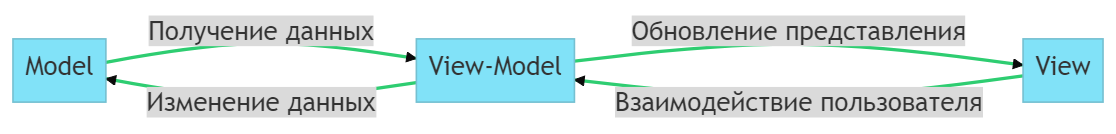
\includegraphics[scale=0.5]{inc/mvvm_logic.png}
  \caption{Компоненты MVVM}
  \label{fig:fig01}
\end{figure}

Использование MVVM в данном приложении позволит создать четкую архитектуру, упростить тестирование и обеспечить возможность быстрой адаптации к изменениям требований или внедрению новых функций. В результате, разработка приложения станет более эффективной, а сопровождение и модификация кода - менее затратными.